\documentclass[output=paper]{langsci/langscibook} 
\author{Juha Lång\affiliation{University of Eastern Finland}
}
% \chapterDOI{} %will be filled in at production


\abstract{This paper reports the results of two experiments, in which the reception of a subtitled television documentary was examined from the point of view of information acquisition. Experiment 1 consisted of group viewings of a short documentary narrated in Russian and subtitled in Finnish, followed by a comprehension test that included questions about the visual elements of the video and details that were mentioned in both the narration and the subtitles. Participants were Finnish natives with no knowledge of Russian, and Russian natives with good Finnish skills. In Experiment 2 the comprehension testing was paired with eye tracking methodology, and the participants were Finnish natives with no Russian language skills and Russian natives with no Finnish language skills. The results showed that the participants who could follow both the narration and the subtitles performed significantly better in the subtitle-related questions. This indicates that the availability of two overlapping information channels enhanced the acquisition of information. Experiment 2 also showed that, compared to the Russian participants, the Finnish participants performed equally well in both types of questions. In conclusion, it seems that subtitles are an effective channel for acquiring information from subtitled television programmes and they do not distract a viewer who is accustomed to them from following also the image.}

\title{Subtitles vs. narration: {T}he acquisition of information from visual-verbal and audio-verbal channels when watching a television documentary}
\rohead{Subtitles vs. narration}
\maketitle

\begin{document}
  

% juha.lang@uef.fi


\section{Introduction}

Reading behaviour has been one of the most researched topics in eye tracking methodology for decades (for a review of the most important findings, see \citealt{Rayner1998, Rayner2009}). The studies have concentrated on so-called normal reading, meaning (usually printed) text on paper. Subtitled television programs differ from this normal condition in many ways that are bound to have an effect on reading behaviour, eye movements and the allocation of attention. The most obvious difference is the presence of multiple information channels \citep{Gottlieb1998}. In addition to the subtitles (visual verbal channel), there is the moving image (visual non-verbal channel) and, usually but not always, an audio track, which can include spoken words (auditive verbal channel) as well as background music and/or sound effects (auditive non-verbal channel). So when reading a book, for example, you can concentrate only on the text and there is only one type of information to process, namely visual verbal information. In contrast, when watching subtitled television programmes there are multiple partially overlapping information channels that battle for the viewer's attention and cognitive resources. This means that the viewer has to integrate the information from the different channels to form a consistent mental model in order to comprehend the contents of the programme. But how effective is this integration?

Studies on using subtitles in language learning (e.g. \citealt{Koolstra1999childrens}; \citealt{Latifi2011}; \citealt{Etemadi2012}; \citealt{Ghia2012}) have shown that subtitles can be an especially effective tool in vocabulary acquisition. \citet{mitterer2009} found that intra-lingual foreign subtitles (i.e. a foreign film subtitled in the language of the film) help speech perception and learning to speak the foreign language, as the foreign words are associated with the proper pronunciation. These findings suggest that some integration of the two types of verbal information happens with beneficial results.

\citet{lee2013} studied how subtitles affect the comprehension of narrative film in a two-part experimental setting. In the first part, they asked a group of native English participants to write down their thoughts while watching a normal (English) or dubbed and subtitled (dubbed into French and subtitled into English) version of a film. In the second part, they asked the participants to sort the events of the film according to their similarity. The results of both experiments showed that the participants who saw the subtitled version made more remarks that referred to earlier events of the film (``bridging inferences'') while the participants who saw the normal version made more remarks that drew from outside the narrative of the film (``elaborations''). Bridging inferences are considered as a sign of local coherence and outside inferences are a sign of global coherence (Albrecht \& O'Brien 1993, referred to in \citealt{lee2013}). The conclusion here was that the viewer's overall comprehension of the film suffered from having to follow the subtitles and the image at the same time.

An earlier study by \citet{lavaur2011} reached similar conclusions. They had a ``3 by 3'' test setting, in which French natives with beginner, intermediate, or advanced English skills, 30 participants per group, saw an English film clip with no subtitles, French (interlingual) subtitles or English (intralingual) subtitles. After seeing the film extract, the participants completed a comprehension test, which included questions requiring recall of verbal information and visual information. The results showed that participants with beginner language skills recalled visual details well when no subtitles were present, but the score went down when subtitles were present. Dialogue recall score naturally went up with the subtitles. In the intermediate language skill group, both the dialogue recall and visual recall scores were largely unaffected by the different subtitling conditions. In other words, the presence or absence of subtitles did not affect the recall of visual details, and the presence of native language subtitles improved the dialogue recall scores only a little. The advanced language skill group got best scores when no subtitles were present in both recall types, and the scores were worst with the French subtitles. \citet{lavaur2011} interpreted this as a proof of the distracting effect of the subtitles, especially when they are unnecessary for comprehension as ``two different types of information are transmitted through the same visual channel (images and subtitles), leading to a competition for cognitive resources'' (ibid.:460). It should be noted, though, that the participants in the study \citet{lavaur2011}, as well as the one by \citet{lee2013}, came from countries that do not use subtitling as the main method of translating foreign films, and thus they were not necessarily accustomed to watching subtitled films. 

In earlier studies, d'Ydewalle and his colleagues came to different conclusions. D'Ydewalle was one of the first researchers to utilize eye tracking in psychological research on watching subtitled programs and reading subtitles (for a review of his early studies, see \citealt{dydewalle1992}). In one of these eye tracking studies, \citet{dydewalle1987} showed participants a German video clip with subtitles in their native tongue. The availability of soundtrack was varied: normal German soundtrack and no soundtrack. Furthermore, some of the participants had a good command of the German language, as they were advanced students of German. A surprising discovery was that the subtitles were read even when the participants understood the language of the soundtrack. This led to two hypotheses: the automaticity hypothesis and the efficiency hypothesis. The first states that reading subtitles is at least partially an automatic process. The second states that information can be acquired more quickly and more efficiently from the subtitles than from the soundtrack. This is because subtitles are read more quickly than the corresponding line is said on the soundtrack. Furthermore, as opposed to the soundtrack, which is heard only once, the subtitles can be re-read in the time frame in which they are visible. 

These hypotheses have been backed up with more recent findings \citep{dydewalle1991, Bruycker2007, Perego2010, Perego2015}. \citet{dydewalle1991} conducted two eye tracking experiments in which participants were shown programmes with both the soundtrack and subtitles in their native tongue: in the first experiment the participants were Americans watching an American movie with English subtitles and in the second experiment Dutch natives were shown a Dutch film with Dutch subtitles. The results corroborated the previous hypotheses as both groups spent considerable time reading the subtitles, although they had no obvious reason to do so. The first experiment also refuted the idea that reading subtitles is a learned skill, since the American participants were not used to watching subtitled movies or television programmes.

\citet{Bruycker2007} examined the differences in eye movements of adults and children when reading television subtitles. In this experiment they used reversed subtitling as one variable condition, i.e. the programme's soundtrack was in the participants' native tongue but the subtitles were in a foreign language unknown to the participants. The eye tracking data showed that the differences in the reading of subtitles between children and adults are similar to the differences found in normal reading: children make longer fixations and shorter saccades. The automaticity hypothesis was further verified, since the data showed that 26\% of the reversed subtitles were fixated on. Clearly, here the efficiency of subtitles as an information channel could not have been the reason for the reading behaviour, because the participants apparently did not understand the language of the subtitles and so could extract little information from them. 

\citet{Perego2010} used eye tracking with word recognition and visual scene recognition tests to examine cognitive effectiveness of watching subtitled movies. In addition to normal, well-structured subtitles, they included in the stimulus some manipulated two-lined subtitles in which the segmentation of noun phrases (NPs) was syntactically incoherent, i.e. the NP was cut between its parts and the different parts of the NP were located on different lines. Based on previous studies \citep{Perego2008} the ill-segmented NPs should have a negative effect on the processing of the subtitled material, but the results of \citet{Perego2010} did not confirm this hypothesis. The eye tracking data did not show significant differences in reading ill-segmented subtitles compared to well-segmented subtitles, apart from slightly longer mean fixation duration in the subtitle area with ill-segmented subtitles. The recognition tests showed good overall performance and there was no significant trade-off between scene recognition and subtitle recognition. This indicates that despite following the subtitles the participants were able to process the image as well, which is in contrast with the findings of \citet{lee2013} and \citet{lavaur2011}.

In a more recent study, \citet{Perego2015} compared cognitive processing of dubbed and subtitled film using various cognitive measures, including dialogue and visual scene recognition and face-name association. They found that the participants who saw the subtitled version of the film extract slightly out-performed the participants who saw the dubbed version in dialogue recognition and general comprehension of the film, while there was no significant difference in visual scene recognition. 

Text seems to attract attention also in other mediums where pictorial information is presented together with text. For example, \citet{carroll1992} examined college students' eye movements while viewing single-caption cartoons, and found that captions were usually read before an exhaustive examination of the picture. \citet{rayner2001} studied gaze patterns while looking at print advertisements in a test setting, where they asked the participants to imagine that they had just moved to England and were looking to buy either a new car or skin care products. They found that the task had an effect on the participants' gaze patterns. When a participant who was tasked to buy a car or skin care products saw a car or skin care advertisement, his/her eyes moved quickly to the text part of the advertisement and he/she spent considerably longer time reading the text than when looking at other types of advertisements. Images also received less attention in the advertisements that were relevant to the given task compared to other advertisements.

Later \citet{rayner2008} used partly the same advertisements in an eye tracking experiment where they asked participants to either rate how much they liked the advertisements or to evaluate the advertisements' effectiveness. The results showed, in contrast to \citet{rayner2001}, that the participants used more time on the images than on the text. Furthermore, the participants' overall eye movement patterns differed greatly in the two experiments, but this was at least partly caused by differences in the advertisements that were used in the experiment. Nevertheless, \citet{rayner2008} reach the conclusion that both the nature of the advertisement looked at and the observer's goals affect the eye movement patterns when looking at print advertisements. In the test setting of \citet{rayner2008}, the participants were probably mainly seeking factual information about the advertised products, which is more often found in the text than in the image. 

It has been shown in multiple studies that when people look at movies or television the gaze is usually concentrated on the centre parts of the screen. \citet{tosi1997} recorded eye movements of 10 adults while they were watching fiction and non-fiction film clips, including extracts from feature films, scientific documentaries, advertisements and news programs. They found a strong centre-of-screen bias in the eye movement patterns and relatively little difference in the individual scan paths of the participants. Interestingly, the data also showed that textual elements, such as signs, attracted gaze, which is consistent with other findings on subtitle reading \citep{dydewalle1987, dydewalle1991, dydewalle1992}. 

The centre-of-screen bias in gaze paths while watching television has since been verified (see, for example, \citet{goldstein2007}; \citet{brasel2008}). \citet{goldstein2007} showed 20 participants video clips from 6 movies of various genres and recorded the participants' eye movements. Their aim was to examine, how much each participant's eye movement patterns differ, i.e. whether everyone looked at the same places on the screen, and whether there was any variation between age or gender groups. The results showed that most of the time people tend to fixate on a relatively small area, as more than half of the time the fixations fell within an area that was less than 12\% of the full image area. There was some variation, though, as male participants' eye movement patterns were more uniform than those of female participants. A similar difference was found between older and younger participants: there was less variation between older participants than younger participants. 

\citet{brasel2008} had a similar test setting. They created a 24-minute video clip, of which about a little over half consisted of content from a nature documentary and a little less than half was advertisements. They also found that the centre of the screen attracted most of the fixations, and 90\% of the fixations landed inside an area which governed less than 27\% of the image area, confirming previous studies by \citet{tosi1997} and \citet{goldstein2007}. Despite this, a closer frame by frame analysis revealed differences in the gaze paths of participants and the difference seemed to grow slowly over time. In other words, when a scene becomes visible, people tend to make the first fixations to roughly the same places, but as the gaze begins to wander around the image area, the dispersion on the gaze paths of each individual increases. Not surprisingly, the content of the video affects this greatly: in \citet{brasel2008} static ``network bumpers'' (images of television network logos at the start of television programs) attracted the most uniform gaze paths while in advertisements the dispersion was greater. 

The present study has three aims. Firstly, it aims to shed further light on the issue of processing efficiency of subtitles. \citet{Perego2010} have proved that processing of subtitled material is effective and there is no visible trade-off between processing the image and the subtitles. Furthermore, studies of subtitles in language learning (e.g. \citealt{mitterer2009}) have revealed the benefit of parallel processing of overlapping information channels. This leads to the hypothesis that the access of two overlapping information channels should have a beneficial effect on the acquisition of information (Hypothesis 1). Secondly, the efficiency hypothesis \citep{dydewalle1987} is further tested by comparing the acquisition of information from the subtitles and the narration. The hypothesis here is that, following the efficiency hypothesis, subtitles are a more efficient channel of information than narration (Hypothesis 2). Hypothesis 2 is expected to be visible in the data as a difference in the performance in the relevant comprehension questions between the groups that used the two channels as their main channel of information. The third aim is to examine the impact of subtitles on the processing of image. \citet{lavaur2011} concluded that subtitles are a significant distraction, especially for those who do not need them for comprehension purposes, but \citet{Perego2010} found no difference between dubbing and subtitling conditions in visual scene comprehension. In the study by \citet{lavaur2011}, the participants were not familiar with subtitled films, which may have affected the results. Hypothesis 3 is that subtitles do not have a negative effect on the processing of image for viewers who are accustomed to watching subtitled films or television programmes. The study approached these issues in two experiments. Experiment 1 included only comprehension testing, while in Experiment 2 it was combined with eye tracking methodology in order to get a deeper understanding of the cognitive processes while watching subtitled television documentary. This study did not concentrate on eye movements per se, but instead used the eye tracking data as a tool to visualize the participants' behaviour.

\section{Experiments}

The study includes two experiments: 1) group sessions with only the questionnaire; 2) solo sessions with eye tracking. Both use the same video stimulus and the same questionnaire, but the participant groups and procedure differ a little. 

The video stimulus used in both of the experiments is a documentary about the Norwegian explorer and Nobel Peace Prize winner Fridtjof Nansen. The running time of the documentary is approximately 7 minutes. The only audio-verbal element of the documentary is the Russian narration and no dialogue is present. The documentary is subtitled into Finnish, and the subtitles were visible for all participant groups, i.e. the material is exactly the same for everyone. The visual elements consist mainly of black-and-white photos and short acted dramatizations that illustrate points in the story. 

Russian was chosen as the language of the stimulus material for a number of reasons. Firstly, like most Finns, the Finnish participants did not understand Russian, and consequently they had to rely solely on the subtitles in order to understand the narrative. Secondly, in Russia subtitling is a little-used method of translating foreign films, dubbing being the method more frequently used. In other words, Russian people are not used to reading subtitles, which helped to shed light on Hypothesis 3. 

The questionnaire included open-ended short answer questions from three categories according to the channel from which the information for the correct answer was available: image, narration, and subtitles. The questionnaire included 28 questions in total, but only 17 of them were analysed in these experiments. The reason for this is that the questions which concerned the information available only from the narration of the documentary fell out of the scope of these experiments and were thus omitted from the analysis. This meant excluding 9 of the questions. Furthermore, it was discovered in the analysis stage that one of the subtitle-related questions and one of the image-related questions proved to be somewhat ambiguous and thus difficult to analyse, so they were excluded from the analysis. This meant that the analysis presented in this paper was based on 5 image-related questions and 12 subtitle-related questions. 

To be more specific, the image-related questions asked about visual details that were not directly mentioned in either the narration or the subtitles. The narration-related questions asked about details that were not included in the translation, i.e. the subtitles, whereas subtitle-related questions asked about details that were mentioned in both the subtitles and the narration. For example, Nansen had a special ship designed for him for his expedition to the North Pole. The narrator mentions the name of the ship (``Fram'') and the ship is shown in several photographs in the video, but the name is not mentioned in the subtitles. One image-related question asked about the number of masts that the ship had, while a narration-centred question asked the participants to recall the name of the ship. An example of a subtitle-related question would be one where participants were asked about Nansen's favourite school subjects, a detail that was mentioned in both the Russian narration and the Finnish subtitles. The questionnaire was available for the participants in Finnish in Experiment 1, and in Finnish and Russian in Experiment 2.

\subsection{Experiment 1}

\subsubsection{Participants}

The participants of Experiment 1 consisted of 14 native Finnish speakers and 20 native Russian speakers. The Finnish natives were students and staff of the University of Eastern Finland. Most of the Russian natives were students of Petrozavodsk State University, but also included some students and staff of the University of Eastern Finland. The Finnish natives had little or no skills in Russian, and the Russian natives were either studying or had studied Finnish at university level and thus were expected to have sufficient Finnish language skills to be able to understand the subtitles in the stimulus video. The mean age of the groups was 21.5 for the Finnish (SD=0.73) and 23.0 for the Russians (SD=1.24). Both groups were strongly lopsided in terms of gender distribution as there were only 4 males in the Finnish group and 3 males in the Russian group.

\subsubsection{Method}

The data in experiment 1 was collected in several group sessions, which were similar in overall procedure save for one exception, detailed below. The participants were first verbally instructed about the procedure of the test session. They were told in advance that their comprehension of the documentary would be tested after seeing the video. The participants saw the stimulus video in a classroom with a data projector, white screen and sound system. After watching the documentary, the participants completed the written questionnaire. An exception to this procedure was the session that was held at Petrozavodsk State University, where the participants watched the documentary in a computer lab, each on a computer monitor of their own and wearing headphones. Each session took approximately 25 minutes in total.

The questionnaires were analysed binomially in terms of correct answers and the binomial data was compared between the language groups with Pearson's $\chi $²-test with Yates' continuity correction (henceforth $\chi $²-test). Statistical analysis was done using the statistical software package R (version 3.1.0).

\subsubsection{Results}

Figures \ref{lang:fig:1} and \ref{lang:fig:2} below show the percentages of right answers to the questions concerning the image and the subtitles, respectively. For the analysis the questions were grouped according to their type and thus the numbering seen here is not the same as on the questionnaire. 

\begin{figure}[h]
 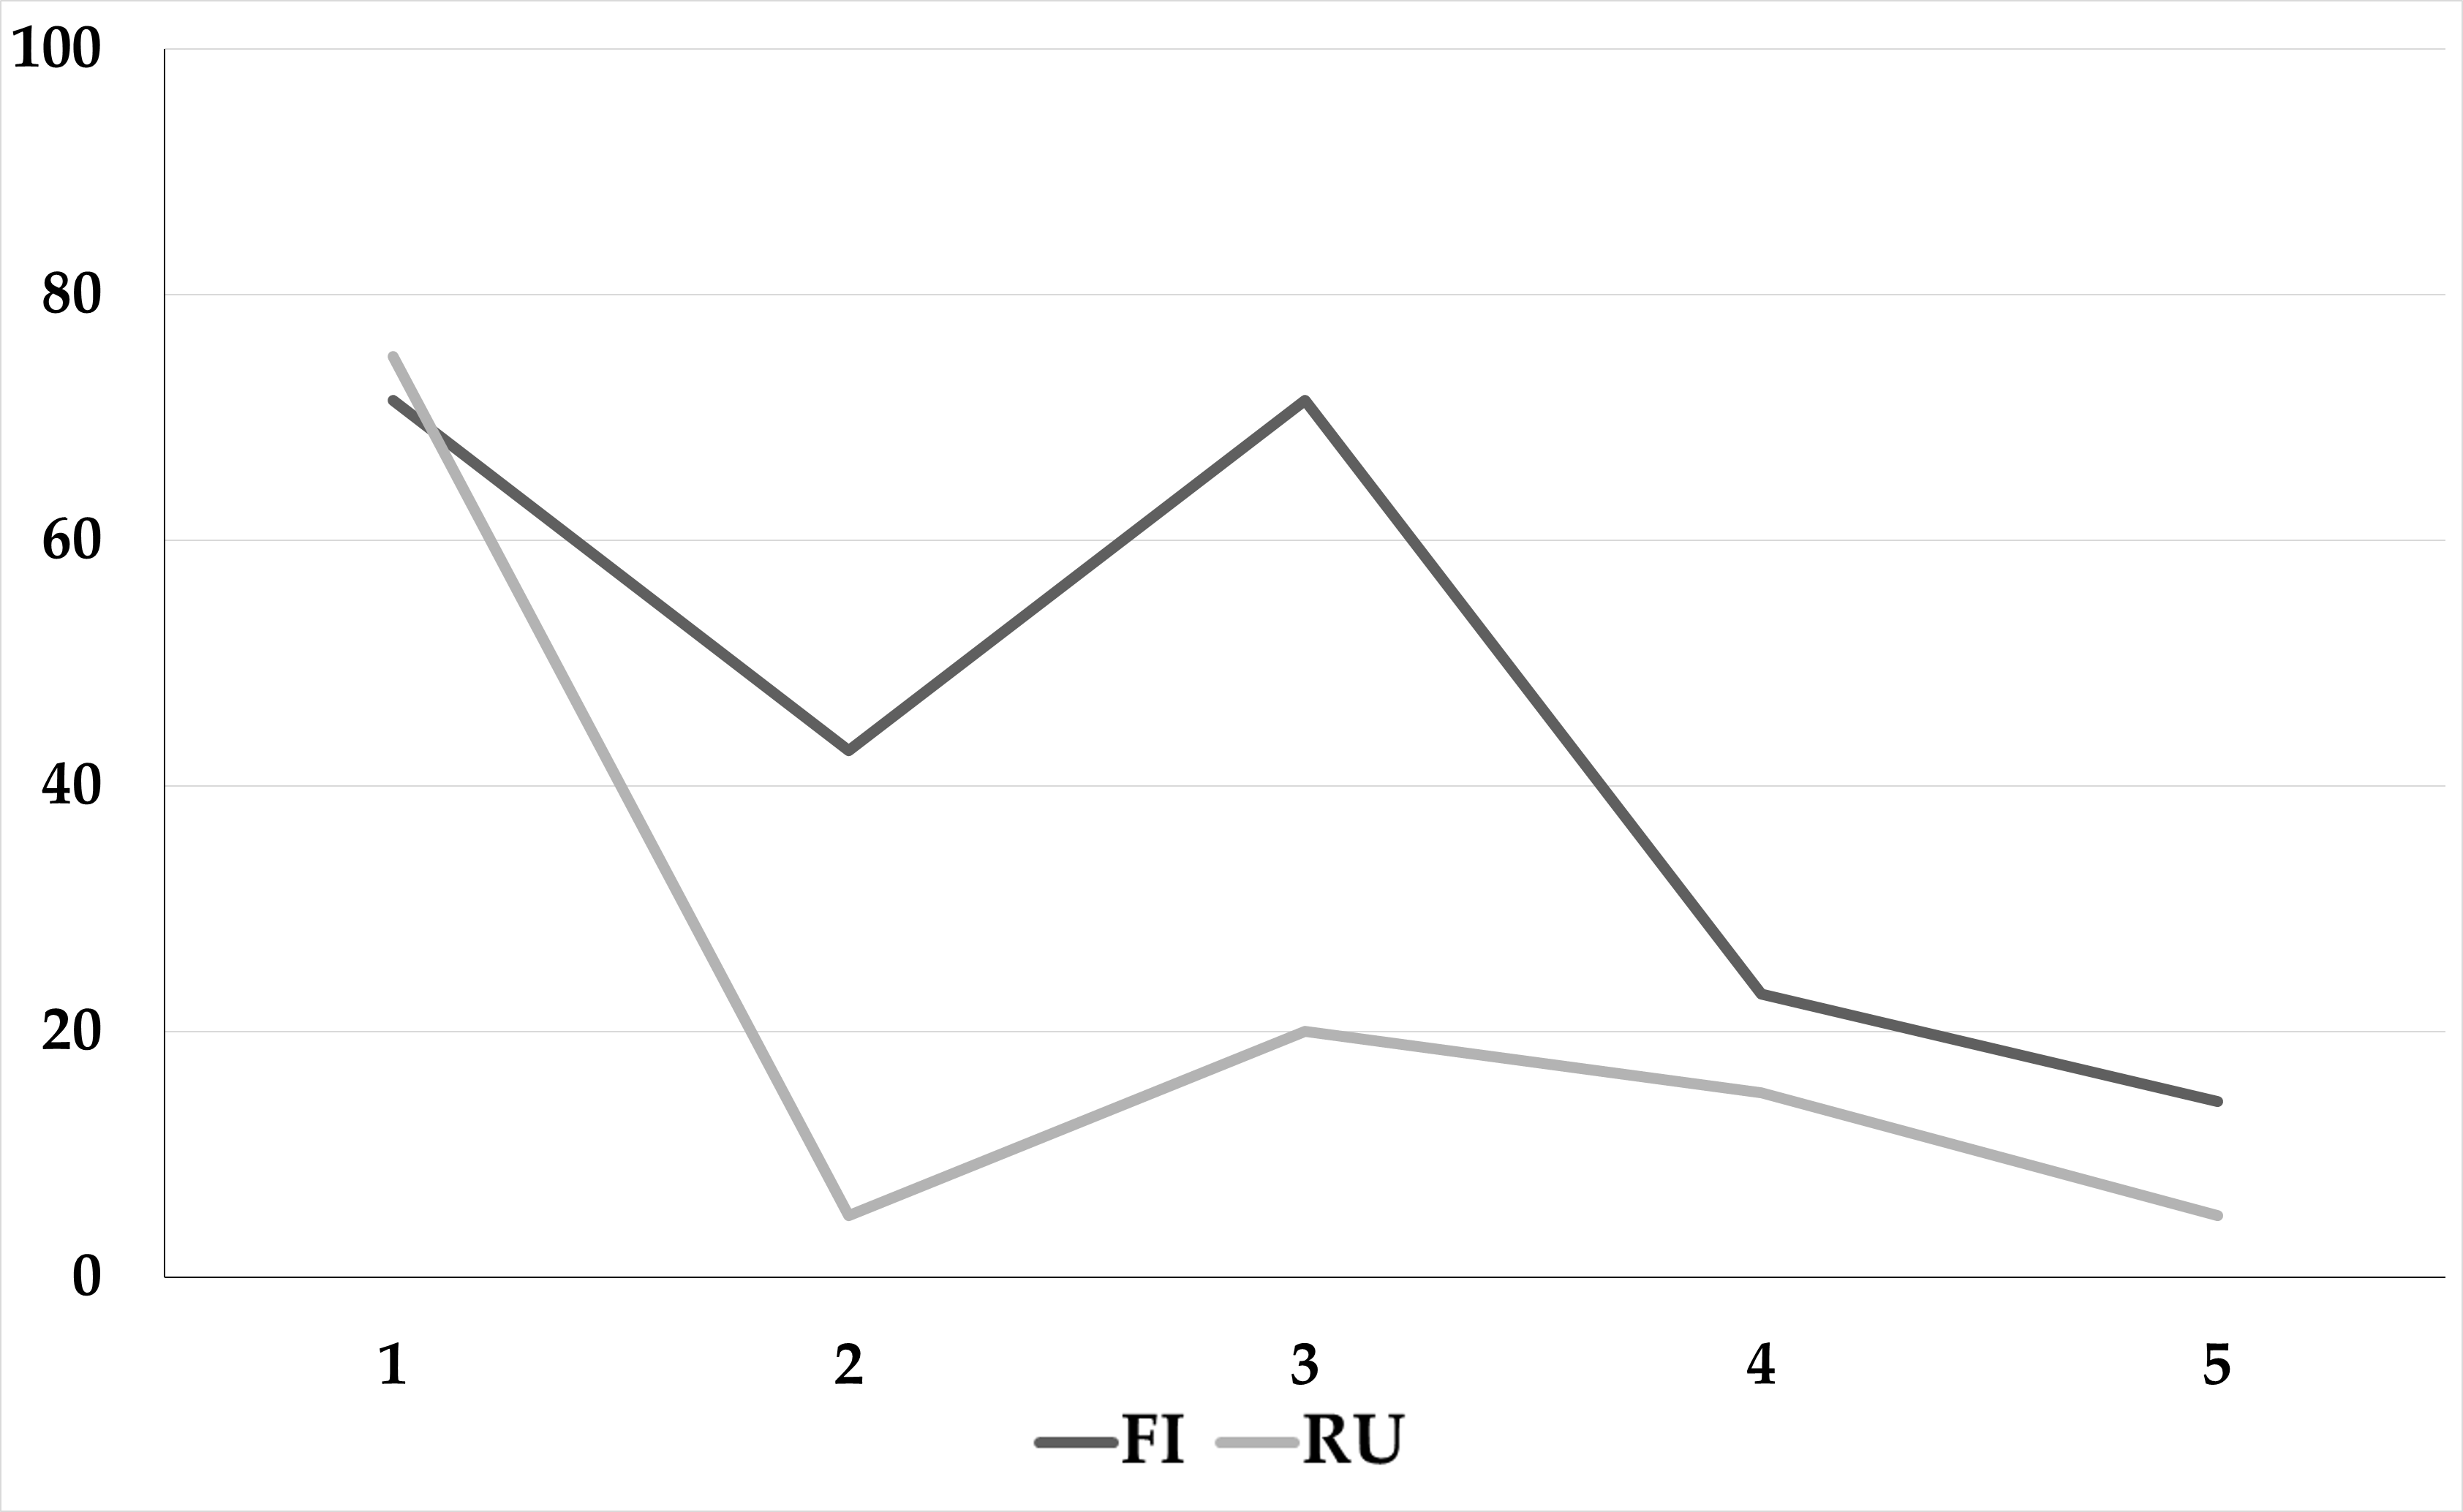
\includegraphics[width=\textwidth]{figures/Lang1.png}
 \caption{The percentage of correct answers in Finnish and Russian groups to the questions (1-5) concerning the image of the stimulus video.}
 \label{lang:fig:1}
\end{figure} 

\begin{figure}[h]
 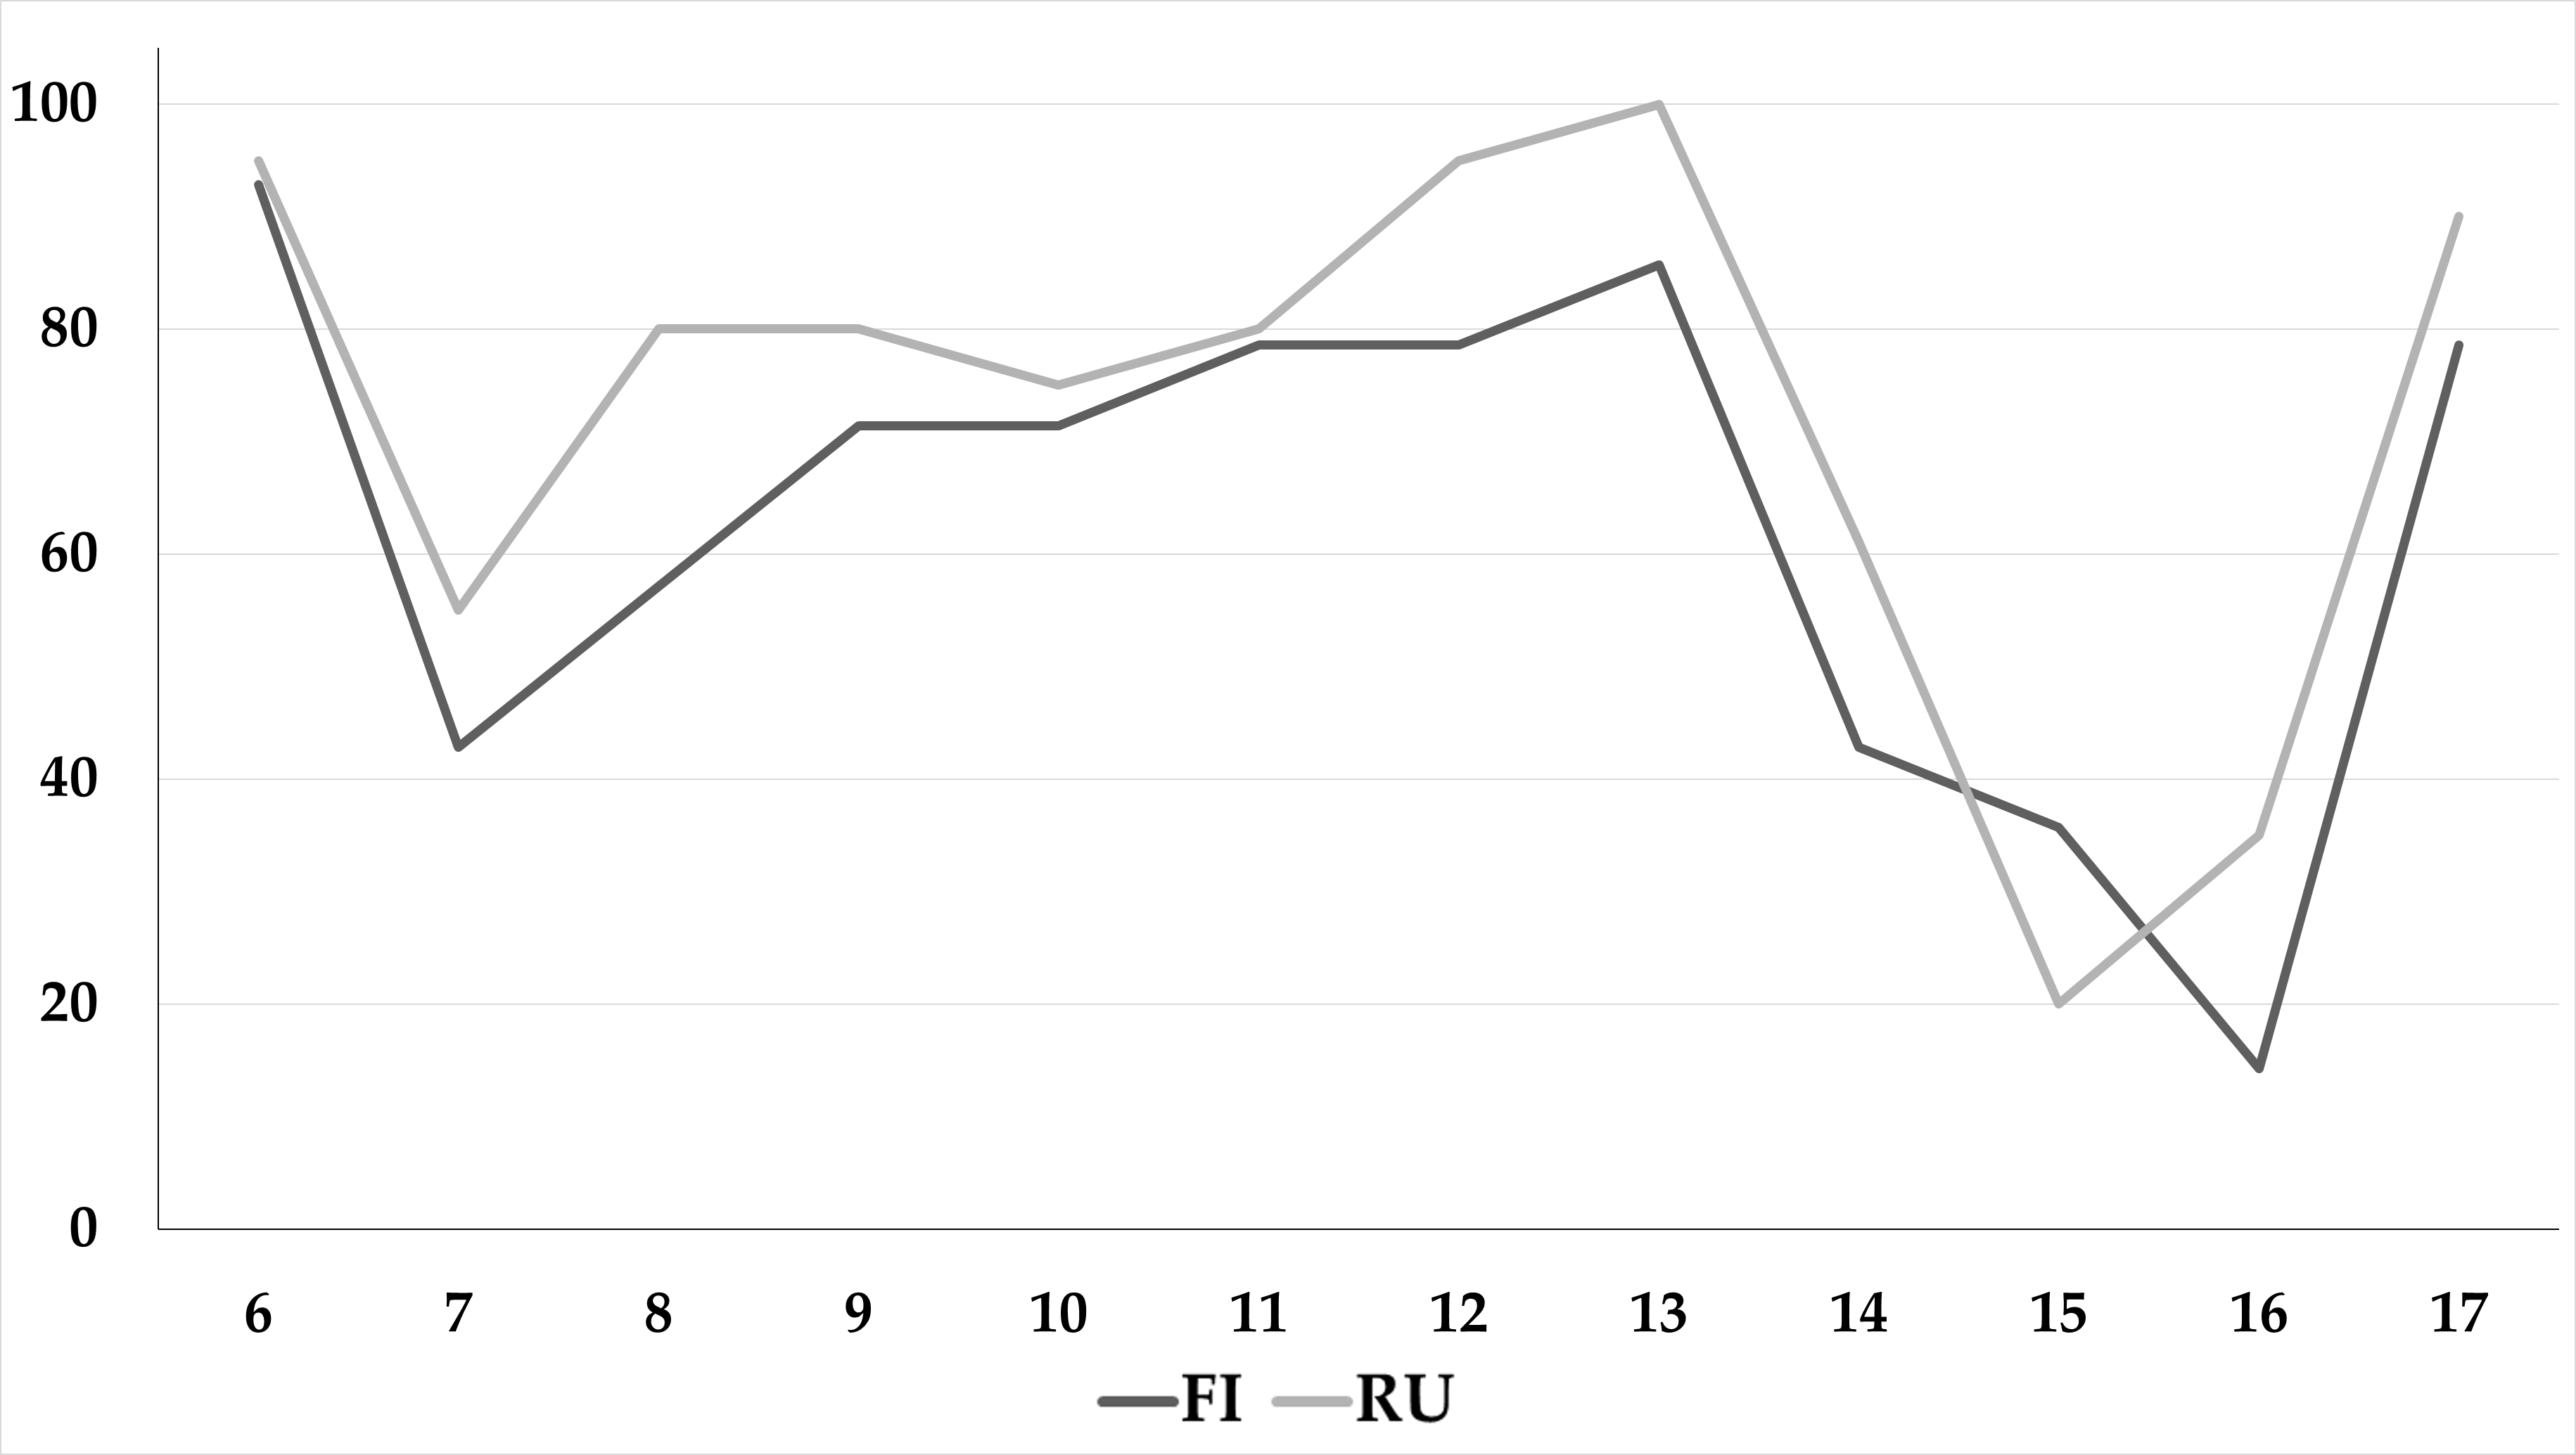
\includegraphics[width=\textwidth]{figures/Lang2.png}
 \caption{The percentage of correct answers in Finnish and Russian groups to the questions (6-17) concerning the subtitles of the stimulus video.}
 \label{lang:fig:2}
\end{figure}



When the image-related and subtitle-related questions were analysed as one group, the overall performances of the Russian and Finnish participants were very even and no statistical difference was visible ($\chi $²(1) = 0.010, p = 0.921). Nevertheless, when the analysis was done separately for the two question groups, differences began to emerge. The Russian participants got slightly better scores than the Finnish participants in the subtitle-related questions (see \figref{lang:fig:2}) and the difference is statistically significant ($\chi $²(1) = 3.90, p = 0.048).  In turn, the Finnish group performed better on the questions concerning the image of the stimulus video (see \figref{lang:fig:1}), and here the difference is also statistically significant ($\chi $²(1) = 7.22, p = 0.007).

\subsubsection{Discussion}

The results of Experiment 1 seem to support the initial hypotheses. The Russian group performed better in almost all of the subtitle-related questions, which confirms Hypothesis 1. It has been shown in previous research \citep{dydewalle1987} that subtitles are usually automatically read when they are available even when they are not necessary for understanding the spoken information. This makes it reasonable to assume that also in this experiment the Russian participants followed, which means that information was absorbed better when the same information came from two overlapping channels, namely, the narration and the subtitles. In light of Paivio's dual-coding theory, which states that presenting verbal information with consistent non-verbal information improves processing and recall \citep{Paivio1986}, the result is as expected. It should be noted, though, that here both of the information channels were verbal, even though they are in two different languages. Nevertheless, the benefit of parallel processing of visual and auditory channels was evident. 

The Finnish group got a noticeably better score in the image-related questions. This result is consistent with Hypothesis 3. Subtitling is the main method of translating foreign films and other television material in Finland, and Finnish people get used to reading subtitles and watching subtitled programmes from an early age. In Russia, dubbing is the preferred method of translating audiovisual material, as is the tendency with major languages. Thus Russian viewers are not accustomed to reading subtitles and they are not as effective as Finnish viewers in processing subtitled audiovisual content. This phenomenon was examined more closely in Experiment 2 with the help of eye tracking methodology.

\subsection{Experiment 2}

Experiment 2 was a continuation of Experiment 1. While Experiment 1 examined the difference in information acquisition between people who could follow only the subtitles and people who could follow both the narration and subtitles, here the goal was to test the difference between people who have access to only one of the information channels. 

\subsubsection{Participants}

The participants of Experiment 2 consisted of 20 Finnish native speakers with little or no Russian skills and 20 Russian speakers. Four participants in the Russian group were omitted from the analysis because they were Russian-Finnish bilingual, and another three because they had good Finnish skills (by their own assessment). This made a total of 13 participants in the Russian group in the analysis of questionnaire data. The data of one Russian participant had to be omitted from the analysis of eye tracking data because of quality issues. The participants were mostly students and staff of the University of Eastern Finland. Again, the gender division was somewhat uneven, since there were only four males in the Russian group and eight males in the Finnish group. The mean ages of the groups were 24.1 (SD = 0.71) for the Finnish group and 31.2 (SD = 4.7) for the Russian group. As can be seen, the Finnish group was fairly homogenous with respect to age variation (age range 19-30) while in the Russian group the variation was larger (age range 17-74). This can be explained by the fact that while the Finnish participant groups only included university students, in order to get a large enough Russian participant group, the invitation to participate in the experiment was not restricted to students only and some non-students also participated. 

\subsubsection{Method}

The biggest differences between Experiment 1 and 2 were the inclusion of eye tracking methodology and the lack of Finnish language skills in the Russian group in Experiment 2. The use of eye trackers also meant that testing had to be done in solo sessions.

The participants' eye movements were tracked with SMI Eye Tracking Glasses 2.0 (SensoMotoric Instruments GmbH, Teltow, Germany), which have a binocular sampling rate of 60 Hz. The data was recorded with SMI iViewETG (version 2.1.0) on a Windows 7 laptop connected to the eye tracking glasses. The video stimulus was shown on a separate computer, an Ubuntu distribution of Linux operating system with a 21-inch LCD display and over-ear headphones to minimize the possibility of distractions. The participant sat on a comfortable office chair, about 60 cm from the display, and the room was normally lit. The test supervisor was present in the room for the whole duration of the recording but had minimum interaction with the participant during the actual recording or when the participant answered the questionnaire. 

Before starting the experiment, the participant received written instructions (available in Finnish and in Russian) that gave a broad outline of what to expect. However, neither the contents of the documentary nor the exact goal of the experiment were revealed. The eye tracking equipment was calibrated with three-point calibration, and the calibration was verified at the start and the end of the recording. The eye movements were recorded only when the participant was watching the documentary. After seeing the video stimulus, the participant was handed the questionnaire and he or she could answer it at his or her own pace. In Experiment 2, the questionnaire was available for the participants in Finnish and in Russian and they could answer it in either of the languages. Typically the session took around 25 minutes in total.

To make the questionnaire data in Experiment 1 comparable with that of Experiment 2, the questions used for the analysis were the same, meaning that one image-related question and one subtitle-related question was omitted from the final analysis. To evaluate the effect of the omissions from the between-group analysis in Experiment 2, the statistical analysis was re-done with the omitted subtitle-related question, but this had no noticeable effect on the results. The questionnaire data was analysed with the $\chi $²-test, as in Experiment 1.

The gaze data was analysed with SMI BeGaze software (version 3.5). The analysis had to be done with the help of a process SMI calls ``semantic gaze mapping'', where gaze data from each recording is manually mapped to selected reference images. By default, the eye tracking glasses use their own scene camera recording as the stimulus video in which they map the gaze data. Mapping all recording data onto reference images via semantic gaze mappings essentially allows an aggregated data analysis of all participants as the analysis can be performed on the mapped reference images instead of the original recordings, each one of which includes data from only one participant. However, the BeGaze software currently does not allow videos to be used as reference stimulus in semantic gaze mapping, which meant that the mappings had to be done onto still screenshots of the documentary. This was not thought to pose a problem here, though, as the analysis is focused on the subtitles, which are a static element by nature. The advantage of the added accuracy of the eye tracking glasses weighted more when choosing the equipment for the experiment.

For the analysis of gaze patterns, the video was divided into scenes of variable lengths. Ten of these scenes were chosen for the analysis. The scenes were analysed as a whole, because the sample sizes in some of the scenes was too small to allow proper statistical analysis. Furthermore, there was no way to divide the scenes into meaningful groups, since all of the scenes consisted of similar audio-visual material (i.e. similar visual material and narration). The length of the chosen scenes varied from approximately 5 seconds to 30 seconds, with a total length of 1 minute and 58 seconds. This covered approximately one fourth of the stimulus video. The first minute and a half was left out of the analysis as an adjustment period. This was thought to give more natural data as the participants get more deeply immersed into the video and forget the experimental nature of the setting. 

The image area was split into two areas of interest (AOIs): the subtitle AOI and image AOI. The eye tracking data of the two AOIs was compared statistically using the Wilcoxon rank sum test with continuity correction in the statistical software package R (version 3.1.0). The analysed metrics were average fixation duration, total dwell time, the number of glances, and fixation count. Average fixation duration is the summed duration of all fixations that land inside an AOI, divided by the number of those fixations. Dwell time equals the sum of all fixations and saccades starting from the first fixation and ending with the last fixation that lands an AOI, i.e. the time spent looking at a specific AOI. Average fixation duration and dwell time are reported in milliseconds. Glances mean the number of saccades that start from outside a specific AOI and end inside the AOI, i.e. the number of times the participant moves his or her gaze into an AOI. Essentially, the glance count helps us determine how often the subtitles were completely skipped. The fixation count is the total number of fixations that the participant made to a specific AOI. In this analysis, all zero values were omitted when analysing dwell times, average fixation durations and fixation counts, meaning that these were analysed only in cases where participants actually looked at the subtitle area.

The Wilcoxon rank sum test assumes that the compared data sets have homogeneous variances, which was achieved in the current data by transforming all dwell times and average fixation times with the common logarithm (log10). The tables below report the actual measured values rather than the transformed values. No transformations were necessary with glance and fixation count data.

\subsubsection{Results}

\paragraph{Questionnaire data}


Figures \ref{lang:fig:3} and \ref{lang:fig:4}, below show the relative number of correct answers in the ET-FI (eye-tracked Finnish) and ET-RU (eye-tracked Russian) groups in questions concerning the image and the subtitles respectively.

\begin{figure}[h]
 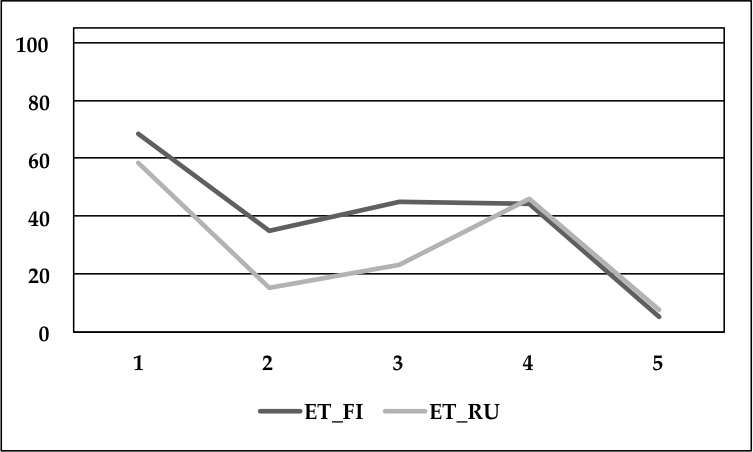
\includegraphics[width=\textwidth]{figures/Lang3.png}
 \caption{The percentage of correct answers in Finnish (ET-FI) and Russian (ET-RU) groups to the questions (1-5) concerning the image of the stimulus video.}
 \label{lang:fig:3}
\end{figure} 

\begin{figure}[h]
 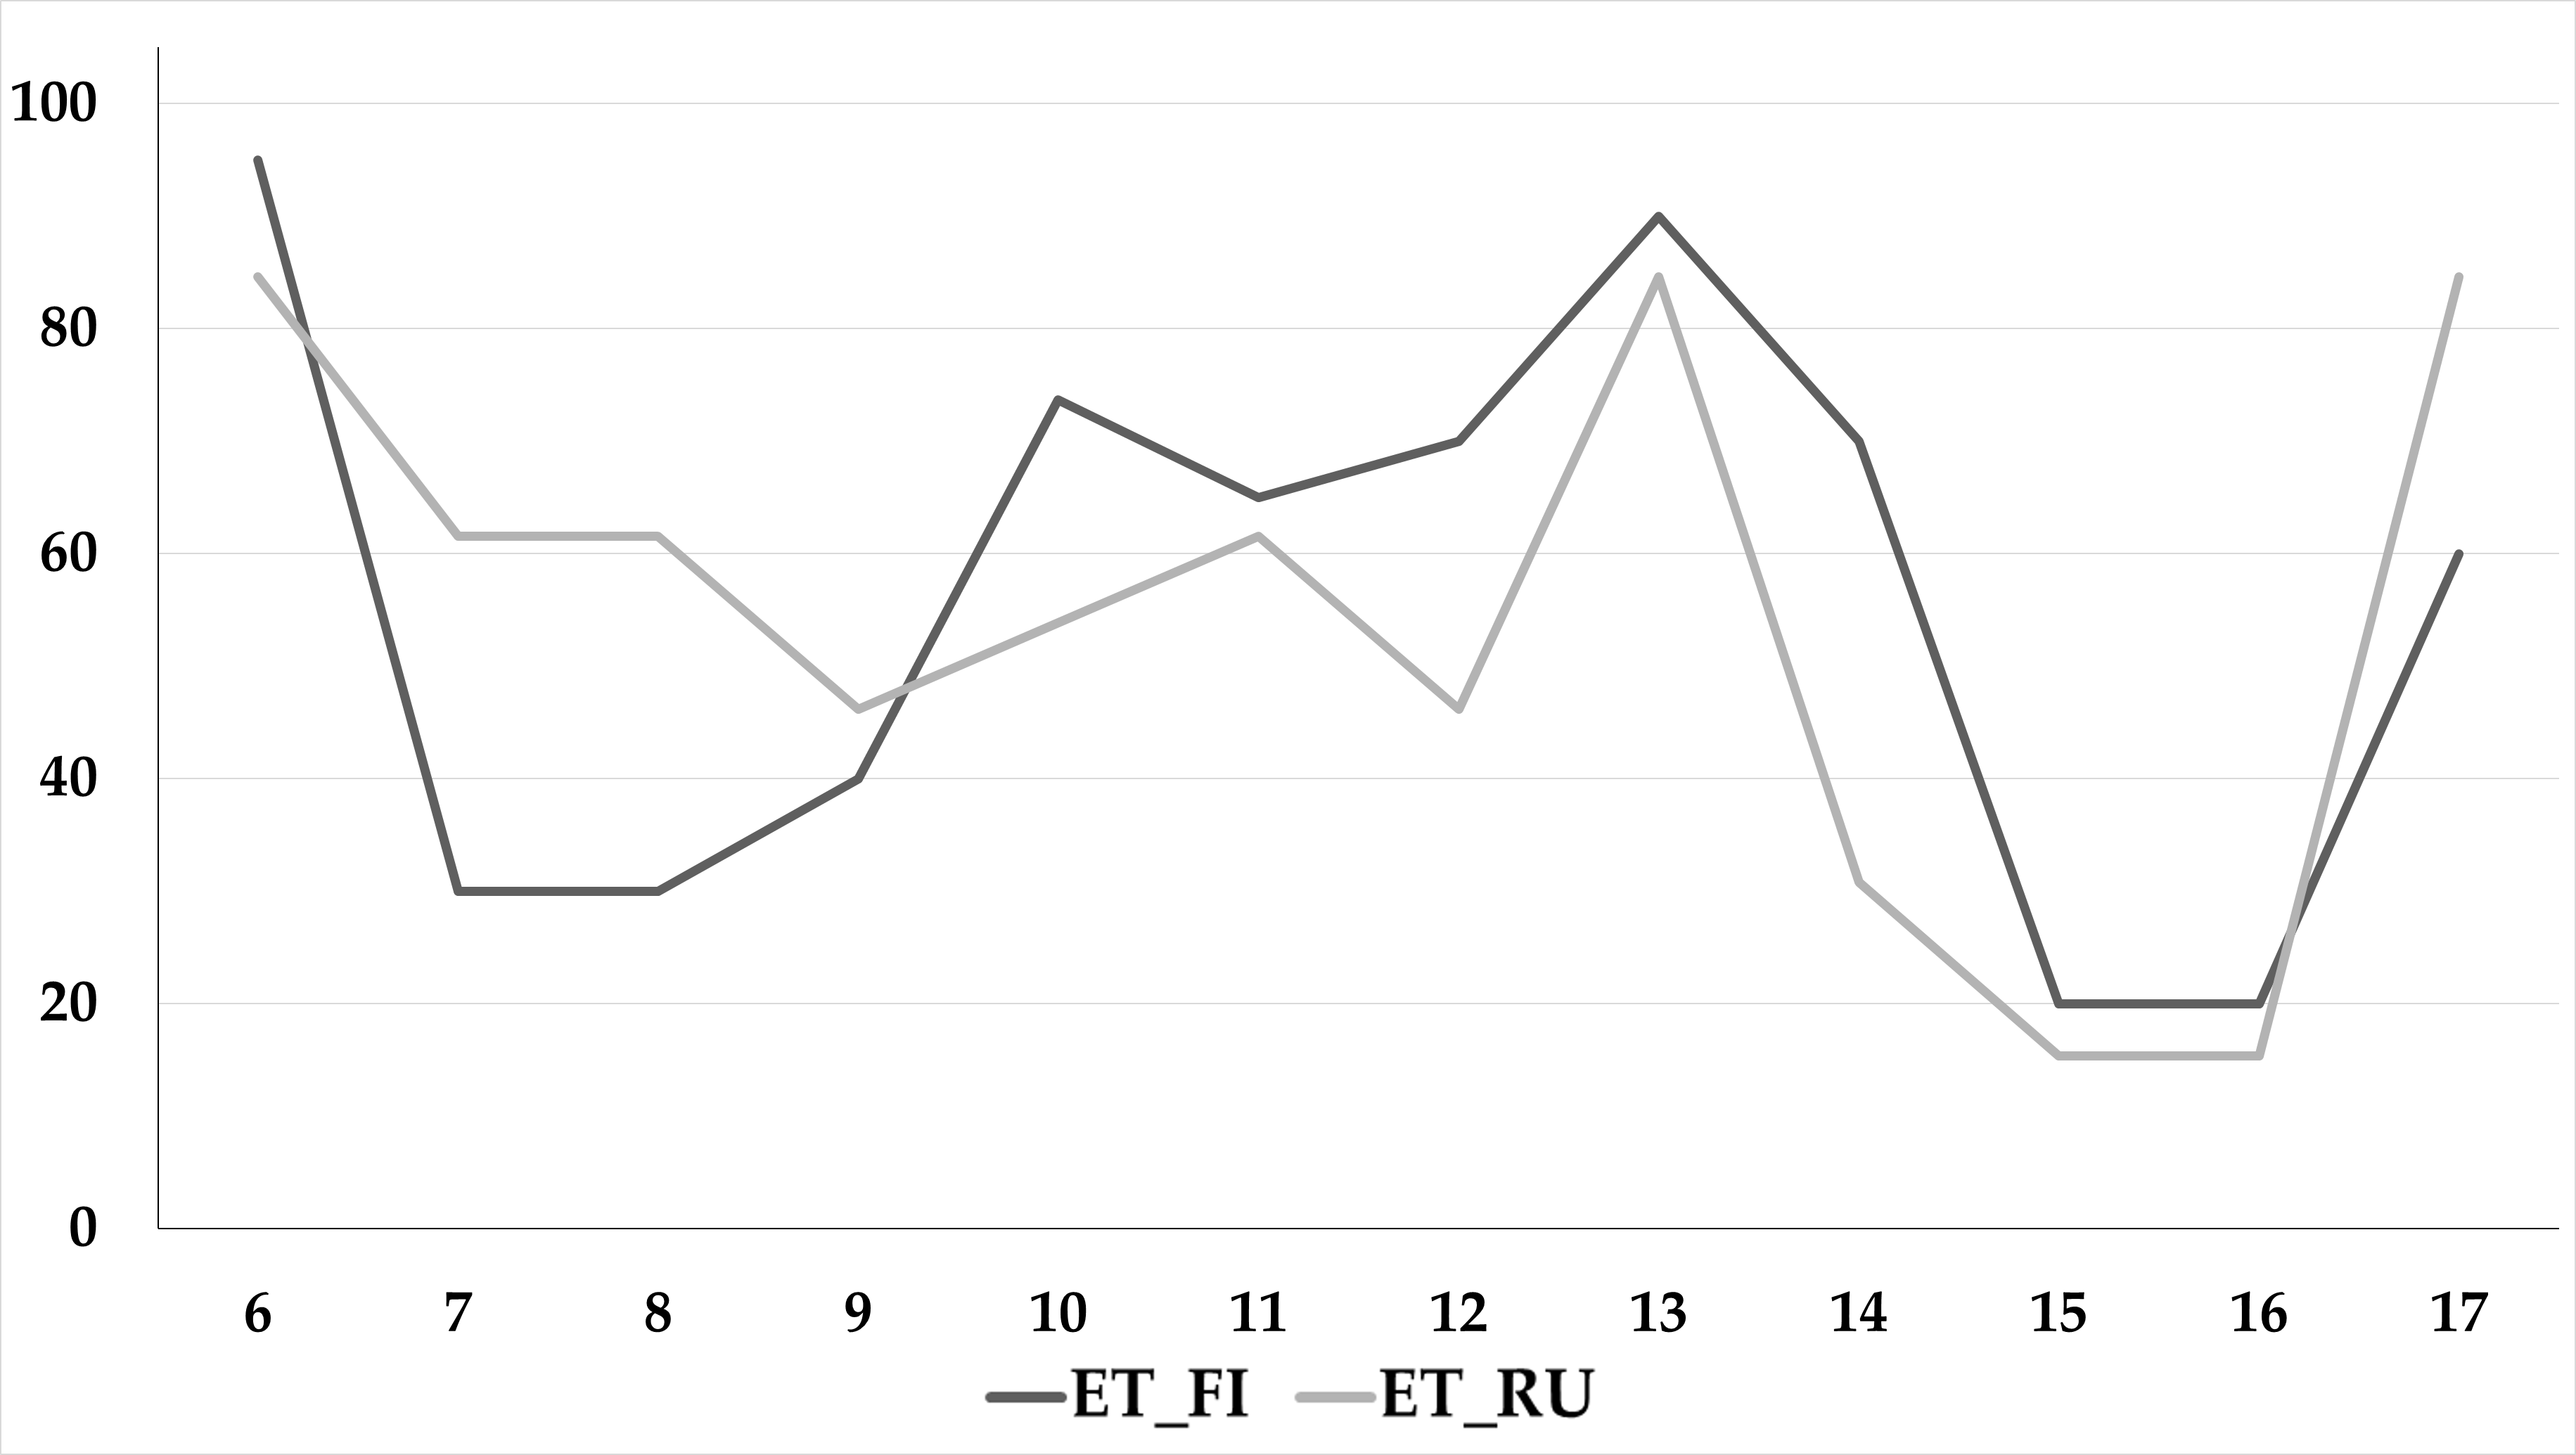
\includegraphics[width=\textwidth]{figures/Lang4.png}
 \caption{The percentage of correct answers in Finnish (ET-FI) and Russian (ET-RU) groups to the questions (6-17) concerning the subtitles of the stimulus video.}
 \label{lang:fig:4}
\end{figure} 

Similarly to the results in Experiment 1, when both types of questions were analysed together, there was no statistically significant difference in the overall performances of the two participant groups ($\chi $²(1)~=~0.574, p = 0.449). In image questions (see \figref{lang:fig:3}), the Finnish group got better scores in almost all questions, again as in Experiment 1, but this time the difference was much smaller and the difference in the overall score did not reach statistical significance ($\chi $²(1)~=~1.24,~p = 0.266). The results in the subtitle questions (see \figref{lang:fig:4}) were more inconsistent across the individual questions, and the overall performance between the groups was similar and no statistical significance was evident ($\chi $²(1)~=~0.028,~p = 0.868). When each question was analysed individually, none of the questions had statistically significant difference  between the groups, but one was close to the level of significance (question 23, $\chi $²(1)~=~3.44,~p = 0.064).

The stimulus and questionnaire were the same in both of the experiments, and this allowed a comparison of the Russian groups. In questions concerning the image, the difference was not statistically significant ($\chi $²(1)~=~0.392,~p~=~0.531, respectively), but in subtitle questions the difference was highly significant ($\chi $²(1)~=~13.3,~p~{\textless}~0.001). A comparison of the two Finnish groups revealed no statistical differences in either types of questions ($\chi $²(1) = 0.277, p = 0.600 in image-related questions and $\chi $²(1) = 1.33, p = 0.248 in subtitle-related questions). Since the Finnish groups were identical in terms of language skills and thus their performance was also expected to be identical, this shows that the different experimental settings did not have a significant impact on the results.

\paragraph{Eye tracking data}

\tabref{lang:tab:1} (below) shows the descriptive statistics for the number of glances into the subtitle area as well as the average dwell times, fixation durations, and fixation counts in the Finnish and Russian groups. The data shows that the Russian participants made significantly less glances to the subtitle area compared to the Finnish group (W~=~101932.5, p {\textless} 0.001). They also skipped the subtitles completely in approximately 64\% of the cases, while the Finnish participants skipped subtitles only in approximately 21\% of the cases. Furthermore, when they looked at the subtitle area, the Russian groups' dwell times were shorter and fixation durations were longer compared to the Finnish groups, and the Russian participants made fewer fixations to the subtitle area. All of these differences were statistically very significant (dwell time: W = 63376.5, p {\textless} 0.001; average fixation duration: W = 38655.5; p {\textless} 0.001, fixation count: W= 60634.0, p {\textless} 0.001). Standard deviations and ranges in the dwell times were quite large in both groups, indicating high variation between individual participants.


\begin{table}
\small
\begin{tabularx}{\textwidth}{Xrrrrcrrr} 
\lsptoprule
& \multicolumn{4}{c}{ FI-ET} && \multicolumn{3}{c}{ RU-ET}\\
				& mean & sd & min & max && mean & sd & min\\
\midrule
{ Glances} 			& 1.02 	  & 0.71   & 0.00 & 4.00     && 0.43   & 0.63   & 0.00\\ \\
{ Dwell time (ms)} 		& 1129.17 & 811.75 & 99.30 & 4192.90 && 796.67 & 667.11 & 98.80\\ \\
{ Average Fixation duration (ms)}	& 157.72  & 71.61  & 74.90 & 732.80  && 172.77 & 60.34  & 77.60\\ \\
{ Fixation count} 		& 4.46    & 2.8    & 1.00  & 17.00   && 3.59   & 2.65   & 1.00\\  
\lspbottomrule
\end{tabularx}
\caption{Descriptive statistics for the number of glances, total dwell times (ms), average fixation duration (ms) and fixation count in the subtitle area for the Finnish and Russian groups.}
\label{lang:tab:1}
\end{table}

\subsubsection{Discussion}

The questionnaire data confirmed some of the findings that were discovered in Experiment 1. In Experiment 2, each group got a similar overall score in the subtitle questions although there was some variation between individual questions. This suggests that, since the same information was available in both channels but the participants in the different groups could only effectively follow one of the channels, both types of verbal channels -- the visual-verbal and audio-verbal channel -- are equally effective as channels for acquiring information. Although this refutes Hypothesis 2, it also demonstrates that the subtitles area is as effective an information channel as the narration. This result is consistent with the results by \citet{Perego2010} and can be seen as further proof for the efficiency hypothesis \citep{dydewalle1987}. 

Nevertheless, when the Russian group in Experiment 1 was compared to the Russian group in Experiment 2, the difference in scores was noticeable in favour of Experiment 1. This suggests that the possibility to follow both the narration and the subtitles gave them a significant advantage, and the redundant information channels enhanced the acquisition verbal of information, confirming Hypothesis 1. A similar effect has been found previously in studies examining language learning while watching subtitled films. \citet{mitterer2009}, for example, found out that watching a foreign language programme with intra-lingual subtitles (redundant audio and visual verbal channels) enhanced viewers' perception of speech. 

The eye tracking data revealed, quite unsurprisingly, that the Finnish group made significantly more glances to the subtitle area than the Russian group. Furthermore, the Russian participants completely skipped over 60\% of the subtitles, but when they did look at the subtitles they made longer but significantly fewer fixations than the Finnish participants. In comparison, Finnish participants skipped on average one of every five (21\%) subtitles. The average fixation duration in normal reading of Finnish is approximately 250 milliseconds and the typical range is 100-500 milliseconds \citep{hyona1996}, and the values are similar to normal reading of English \citep{Rayner1998}. \citet{Bruycker2007} reported adults' average fixation durations in standard (interlingual) subtitles as 178 milliseconds in one-lined subtitles and 179 milliseconds in two-lined subtitles. The averages reported here follow the same pattern: the average fixation durations of subtitles are shorter (157.72 milliseconds for the Finnish group and 172.77 milliseconds for the Russian group) than in normal reading. The reason for this is possibly the fact that television viewer's reading pace is dictated by the presentation time of the subtitles and, in cases where the viewer misses a subtitle, there is no way to go back. Thus the viewer has to adapt a faster reading strategy to make sure that he/she is able to read, and in cases of confusion possibly re-read, the subtitles. 

Although in Experiment 2 the Finnish group performed better than the Russian group in most of the questions concerning the visual elements of the stimulus material, the difference did not reach statistical significance. In contrast, in Experiment 1 a statistically significant difference was found, with the Finnish group performing noticeably better than the Russian participants, so the results leave some room for speculation. Furthermore, the dwell times in Experiment 2 showed that the Russian group spent less time on the subtitle area than the Finnish group, by a very significant margin. It can be speculated that had the eye movements of the participants in Experiment 1 been tracked, the results would have been different. After all, the Russian participants in Experiment 1 understood the subtitles and most likely followed them more extensively than the Russian participants in Experiment 2.

Examined from another perspective, the difference in the dwell times suggests that, compared to the Finnish group, the Russian participants spent more time looking at the picture, and this was not reflected in the results of the questionnaire. On the contrary, in three of the five image-related questions the Finnish group got better scores than the Russian group. In other words, following subtitles did not have a negative effect on the Finnish groups' scores in the image questions, although reading subtitles drew the participants' attention away from the image. This indicates that reading subtitles is not a noticeable distraction from following the image, at least for people who are used to watching subtitled television programmes, which confirms Hypothesis 3. \citet{Perego2010} made the same conclusion, when they discovered that there was no noticeable trade-off in scene recognition and subtitle recognition when watching subtitled films. In contrast, in Experiment 1 the Russian group performed significantly worse in the image-related questions than the Finnish group. This suggests that the notion of unfamiliarity with subtitled material is at least partially the reason also for the contrasting results by \citet{lavaur2011}, who found a trade-off effect of dialogue vs. visual comprehension with participants who had to rely on the subtitles in order to comprehend the dialogue of the film. Furthermore, they found that in the group who understood spoken dialogue, the visual comprehension score suffered from the presence of subtitles. The analysis in the present paper revealed no significant difference in the performances of the Russian groups in Experiment 1 and Experiment 2 in the image-related questions. This indicates that the subtitles had a similar effect on following the image for all Russian participants, no matter whether they could understand the subtitles or not.

One point worth mentioning is that although the Russian participants in Experiment 2 did not properly understand the language of the subtitles, they still looked at them in 40 percent of the cases. It has been shown that text seems to draw attention naturally in many contexts where it is presented with images, such as advertisements \citep{rayner2001,rayner2008}, and textual elements draw attention also in non-subtitled television material \citep{tosi1997}. The automaticity hypothesis introduced by \citet{dydewalle1987} stated that reading subtitles is an automated process, and it has been proven to be true even when viewers are not accustomed to watching subtitled programmes \citep{dydewalle1991}. In the present study, the same effect was seen in a case where the participants did not even understand the language of the subtitles. Another explanation is possible here, though. The stimulus material of the present study was a short documentary, which naturally included facts such as numerical dates and important names. The participants knew before watching the video that the post-viewing questionnaire possibly required them to remember some of these facts. They were also often included in the subtitles and, as they were in a sense an inter-lingual element of the subtitles, the Russian participants could have spotted these facts from the text and used this as a memory-enhancing viewing strategy. 

\section{Conclusions}

The aim of this study was to examine the acquisition of information from different information channels present in a subtitled television documentary. There were three hypotheses: 1) the access of two overlapping information channels should have a beneficial effect on the acquisition of information, 2) subtitles are a more efficient channel of information than narration, and 3) subtitles do not have a negative effect on the processing of image for viewers who are accustomed to watching subtitled films or television programmes. The questionnaire results of Experiment 1 and 2 confirmed Hypothesis 1, as in both experiments the access to both subtitles and narration improved the comprehension score, compared to the participants who only had access to one of the information channels. In contrast, Hypotheses 2 was refuted, as there was no visible difference in the performance of the two groups in Experiment 2 with subtitle-related questions. Hypothesis 3 was also confirmed, as the data in Experiment 2 showed no significant differences between the two groups in questions concerning the image, and the difference in Experiment 1 between the Russian and Finnish participants was statistically significant in favour of the Finnish group. 

To summarize, the overlapping information channels can benefit viewers who can access both of them. The question of the effectiveness of the visual verbal and audio verbal channels remains open to debate, as no difference was found in the present study. It seems that subtitles are an effective way of translating foreign material, and those who are familiar with reading subtitles can also follow the image effectively despite following the subtitles. Nevertheless, it should be remembered that subtitles are bound by strict spatial and temporal constraints, and usually the original message has to be simplified and/or condensed as there simply is not enough time or space to include everything in the subtitles. Hence the role of the translator is an important one, because he or she ultimately decides what pieces of information are the most important to be conveyed and what can be left out. These experiments did not address the issue of emotional and aesthetic effects that subtitles have on the viewing experience, a viewpoint which could bring a new aspect to the discussion on audiovisual translation (AVT), especially when comparing dubbing and subtitling. Furthermore, in the stimulus material here the subtitles were done in accordance with the subtitling conventions, which ensured that the subtitles were formatted and paced so that they were easy to read and the participants had enough time to read them. In future, research into the validity of these conventions for cognition and reception could prove to be a beneficial approach in the study of audiovisual translating.

% \section{References}
% 
% 
% Brasel, S. Adam and James Gips. 2008. “Points of view: Where do we look when we watch TV?” \textit{Perception} 37:1890-1894.
% 
% 
% 
% Carroll, Patrick, Young, Jason R. and Michael S. Guertin. 1992. “Visual Analysis of Cartoons: A View from the Far Side”. In \textit{Eye Movements and Visual Cognition: Scene Perception and Reading,} edited by Keith Rayner, 444-461
% 
% 
% 
% d’Ydewalle, Géry and Ingrid Gielen. 1992. “Attention Allocation with Overlapping Sound, Image, and Text”. In \textit{Eye Movements and Visual Cognition: Scene Perception and Reading,} edited by Keith Rayner, 415-427. New York: Springer-Verlag.
% 
% 
% 
% d’Ydewalle, Géry, Praet, Caroline, Verfaille, Karl and Johan Van Rensbergen. 1991. “Watching Subtitled Television: Automatic Reading Behavior”. \textit{Communication Research }18(5):540-666.
% 
% 
% 
% d’Ydewalle, Géry, Van Rensbergen, Johan and Joris Pollet. 1987. “Reading a message when the same message is auditorily available in another language: The case of subtitling”. In \textit{Eye movements: From physiology to cognition, }edited by J.K. O’Regan and A. Lévy-Schoen,\textit{ }313-321. Amsterdam: Elsevier Science.
% 
% 
% 
% d’Ydewalle, Géry and Wim De Bruycker. 2007. “Eye Movements of Children and Adults While Reading Television Subtitles”. \textit{European Pyschologist} 12(3):196-205.
% 
% 
% 
% Etemadi, Aida. 2012. “Effects of Bimodal Subtitling of English Movies on Content Comprehension and Vocabulary Recognition”. \textit{International Journal of English Linguistics} 2(1):239-248.
% 
% 
% 
% Goldstein, Robert B., Woods, Russell L., and Eli Peli. 2007. “Where people look when watching movies: Do all viewers look at the same place?” \textit{Computers in Biology and Medicine }37:957-964.
% 
% 
% 
% Gottlieb, Henrik. 1998. “Subtitling”. In \textit{Routledge Encyclopedia of Translation Studies}, edited by Mona Baker, 244-348. London: Routledge.
% 
% 
% 
% Hyönä, Jukka. 1996 “Silmänliikkeet lukemisessa [Eye movements in reading]”. In \textit{Mieli ja aivot: Kognitiivinen neurotiede [Mind and brain: Cognitive neuroscience],} edited by Revonsuo, Antti, Lang, Heikki and Olli Aaltonen, 283-292. Turku: Centre for Cognitive Neuroscience, University of Turku.
% 
% 
% 
% Koolstra, Cees M., and Johannes W. J. Beentjes. 1999. “Children's Vocabulary Acquisition in a Foreign Language through Watching Subtitled Television Programs at Home”. \textit{Educational Technology Research and Development} 47(1):51-60.
% 
% 
% 
% Latifi, Mehdi, Mobalegh, Ali and Elham Mohammadi. 2011. “Movie Subtitles and The Improvement of Listening Comprehension Ability: Does it help?” \textit{The Journal of Language Teaching and Learning} 1(2):18-29. 
% 
% 
% 
% Lavaur, Jean-Marc, and Dominique Bairstow. 2011. “Languages on the screen: Is film comprehension related to the viewers’ fluency level and to the language in the subtitles?” \textit{International Journal of Psychology} 46(6):455-462. 
% 
% 
% 
% Lee, Mina, Roskos, Beverly and David R. Ewoldsen. 2013. “The Impact of Subtitles on Comprehension of Narrative Film”. \textit{Media Psychology} 16:412-440. 
% 
% 
% 
% Mitterer, Holger and James M. McQueen. 2009. “Foreign Subtitles Help but Native-Language Subtitles Harm Foreign Speech Perception”. \textit{PLos ONE }4(11):e7785.
% 
% 
% 
% Paivio, Allan. 1986. \textit{Mental Representations: A Dual Coding Approach}. New York: Oxford University Press.
% 
% 
% 
% Perego, Elisa. 2008. “What Would We Read Best? Hypotheses and Suggestions for the Location of Line Breaks in Film Subtitles”.  \textit{The Sign Language Translator and Interpreter} 2(1):35-63.
% 
% 
% 
% Perego, Elisa, Del Missier, Fabio, and Sara Bottiroli. 2015. “Dubbing versus subtitling in young and older adults: cognitive and evaluative aspects”. \textit{Perspective: Studies in Translatology }23(1):1-21\textit{.}
% 
% 
% 
% Perego, Elisa, Del Missier, Fabio, Porta, Marco and Mauro Mosconi. 2010. “The Cognitive Effectiveness of Subtitle Processing”. \textit{Media Psychology} 13:243-272.
% 
% 
% 
% Rayner, Keith. 2009. “Eye movements and attention in reading, scene perception, and visual search”. \textit{The Quarterly Journal of Experimental Psychology} 62(8):1457-1506.
% 
% 
% 
% Rayner, Keith, Miller, Brett and Caren M. Rotello. 2008. “Eye movements when looking at print advertisements: the goal of the viewer matters”. \textit{Applied Cognitive Psychology} 22(5):697-707.
% 
% 
% 
% Rayner, Keith, Rotello, Caren M., Stewart, Andrew J., Keir, Jessica and Karen A. Duffy. 2001. “Integrating Text and Pictorial Information: Eye Movements When Looking at Print Advertisements”. \textit{Journal of Experimental Psychology: Applied} 7(3):219226.
% 
% 
% 
% Tosi, Virgilio, Mecacci, Luciano and Elio Pasquali. 1997. “Scanning Eye Movements made when Viewing Film: Preliminary Observations”. \textit{International Journal of Neuroscience} 92(1-2):47-52.


%\subsection*{Abbreviations}
\subsection*{Acknowledgements}
The author would like to thank Anna Petrova, from Petrozavodsk State University, for assistance in data collection, as well as the two anonymous reviewers for their valuable comments.
\printbibliography[heading=subbibliography,notkeyword=this]

\end{document}